\documentclass[usenames,dvipsnames]{beamer}
\usetheme{Boadilla}
\usepackage{hyperref}
\usepackage{tikz}
\usetikzlibrary{shapes,positioning}
\usepackage{graphicx}
\usepackage{fontawesome}
\usepackage{fancyvrb}
\usepackage{adjustbox}
\usepackage{multicol}
\usepackage{subfig}
\usepackage{xcolor}
\usepackage{optparams}
\usepackage{xstring}
\usepackage[
    backend=biber, 
    natbib=true,
    style=numeric,
    sorting=none,
    style=verbose-ibid,
]{biblatex}
\addbibresource{citations.bib}
\usepackage{pgfpages}
\definecolor{ao(english)}{rgb}{0.0, 0.5, 0.0}
\definecolor{burgundy}{rgb}{0.5, 0.0, 0.13}
\setbeameroption{show notes}
\setbeameroption{show notes on second screen=right}
%\setbeameroption{hide notes}

\def\footshortciteintern[#1][#2]#3{%
\ifx#1\empty 
% Nur Autor
\footnote{\citeauthor{#3}, \citeyear{#3}.}
\else
\ifx#2\empty
% Autor und Seite
\footnote{\citeauthor{#3}, \citeyear{#3}, #1.}
\else
% Autor, Seite und vgl.
\expandafter  
\footnote{\citeauthor{#3}, \citetitle{#3}, \citeyear{#3}, \citeurl{#3}.}
\fi
\fi
}
\newcommand*\footshortcite{%
\optparams{\footshortciteintern}{[\empty][\empty]}
}
\newcommand*\footmediumcite{%
\optparams{\footshortciteintern}{[][]}
}


\title{Structured sparsity}
\author{Sevag Hanssian}
\date{March 25, 2021}
\institute{MUMT 622, Winter 2021}
\setbeamertemplate{navigation symbols}{}

\begin{document}

\begin{frame}
\maketitle
\end{frame}

\begin{frame}
	\frametitle{Structured sparsity}
	\begin{itemize}
		\item
			Main paper: \citet{sparsitykowalski}
		\item
			Same year, same authors: \citet{sparsitykowalski2}
		\item
			Same techniques: \citet{wmdct}
	\end{itemize}
\end{frame}

\begin{frame}
	\frametitle{Sparsity}
	\begin{quote}
		Sparsity seems to be a particularly efficient guiding principle in view of a number of tasks such as signal compression, denoising, image deblurring, blind source separation, ... The guiding principle may be summarized as follows: for most signal classes, it is possible to find a basis or a dictionary of elementary building blocks (or atoms) with respect to which all (or most) signals in the class may be expanded, so that when the expansion is truncated in a suitable way, high precision approximations are obtained even when very few terms are retained.\footshortcite{sparsitykowalski}
	\end{quote}
\end{frame}

\begin{frame}
	\frametitle{LASSO shrinkage}
	\citet{tibshirani} proposed a new technique for linear regression: LASSO (least absolute shrinkage and selection operator). It ``minimizes the usual sum of squared errors, with a bound on the sum of the absolute values of the coefficients.''\footnote{\url{https://statweb.stanford.edu/~tibs/lasso.html}}
	\begin{figure}
		\vspace{-0.5em}
		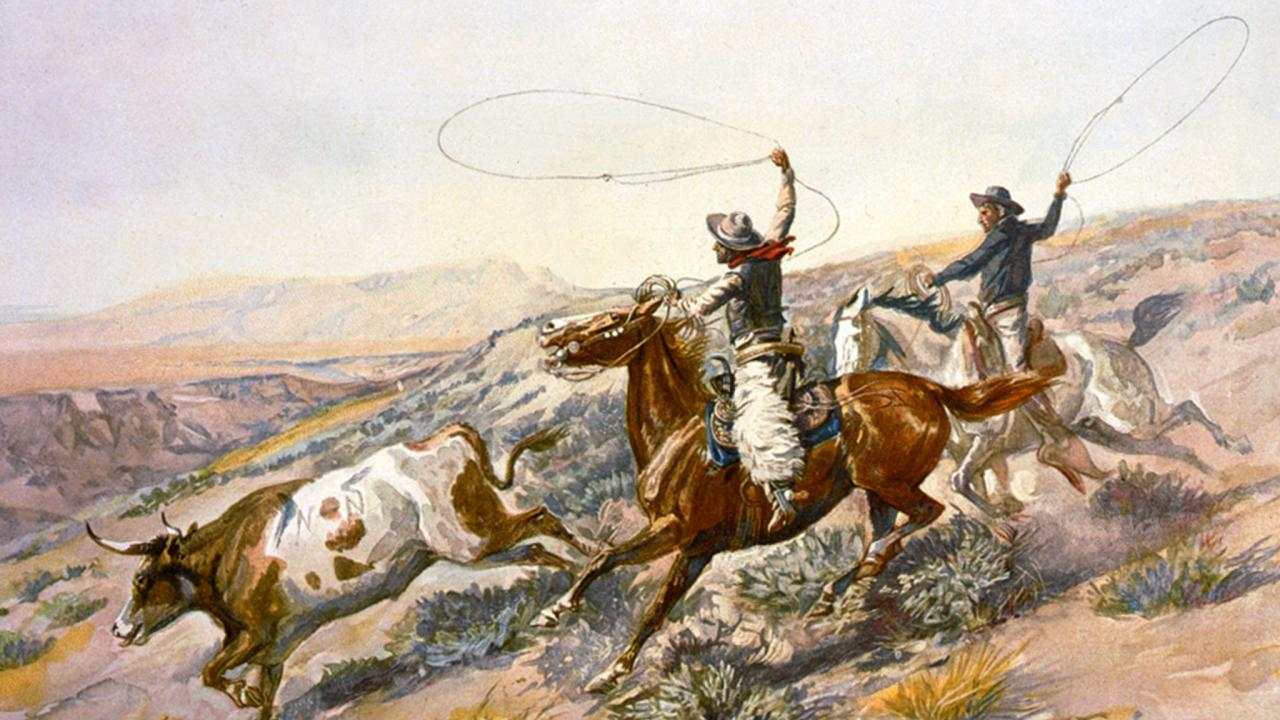
\includegraphics[width=5cm]{./lasso.jpg}
		\caption{Lasso is an acronym and also an analogy for cattle ranchers\footfullcite{tibshirani2}}
	\end{figure}
\end{frame}

\begin{frame}
	\frametitle{Similar ideas -- basis pursuit}
	\begin{quote}
		Basis pursuit (BP) is a principle for decomposing a signal into an ``optimal'' superposition of dictionary elements, where optimal means having the smallest l1 norm of coefficients among all such decompositions\footshortcite{dictionary1}
	\end{quote}
	Least Squares Optimization with L1 Regularization:\footfullcite{Schmidt05leastsquares}
	Estimating Least Squares parameters subject to an L1 penalty was presented and popularized independently under the names Least Absolute Selection and Shrinkage Operator (LASSO) in \citet{tibshirani}  and Basis Pursuit Denoising in \citet{dictionary2}
\end{frame}

\begin{frame}
	\frametitle{L1 and L2 norm}
	Problem to solve:
	\begin{itemize}
		\item
			Given $\mathbf{y} \in \mathbb{R}^{T}$ be a noisy representation of a signal $\mathbf{s} \in \mathbb{R}^{T}$
		\item
			Let $\mathcal{D}$ denote a fixed dictionary for $\mathbb{R}^{T}$, and denote by $\mathit{A} \in \mathbb{R}^{T \times N}$ the matrix whose columns are the vectors from dictionary $\mathcal{D}$
		\item
			We assume $\mathbf{s}$ has a sparse expansion in $\mathcal{D}$
		\item
			We want to estimate $\mathbf{s}$ from $\mathbf{y}$
		\item
			LASSO approach: 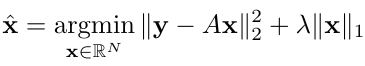
\includegraphics[width=4cm]{./lassol1.png}
		\item
			$A\mathbf{\hat{x}}$ is the estimate of $\mathbf{y}$, $\lambda$ is a fixed parameter
		\item
			L1 norm is the $|| \cdot ||_{1}$ expression
		\item
			Generally, Lp norm is $|| \cdot ||_{p}^{p}$, so L2 norm is $|| \cdot ||_{2}^{2}$
		\item
			These are loss functions for the approximation. Can apply a mixed norm in two dimensions $\mathcal{P}_{p,q}$, e.g., time and frequency
	\end{itemize}
\end{frame}

\begin{frame}
	\frametitle{Mixed norm in time and frequency}
	\begin{multicols}{2}
	In the context of time-frequency dictionaries, a natural step beyond classical sparsity approaches is the introduction of sparsity criteria which take into account the two-dimensionality of the time-frequency representations used. Mixed norms on the coefficient arrays make it possible to enforce sparsity in one domain and diversity and persistence in the other domain.\footfullcite{wmdct}

	\begin{figure}
		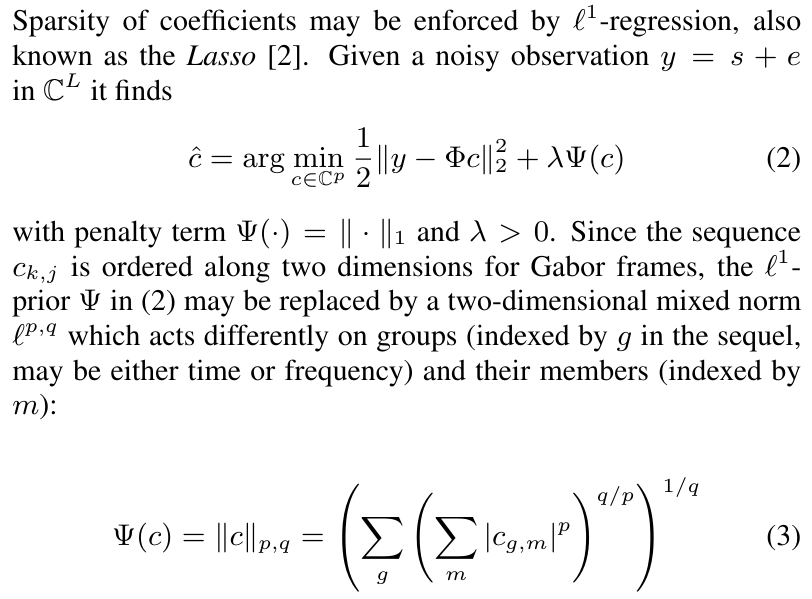
\includegraphics[width=6cm]{./mixednorm.png}
	\end{figure}
	\end{multicols}
\end{frame}

\begin{frame}
	\frametitle{Elitist and Group LASSO}
	Two new and strikingly different shrinkage operators, E-LASSO and G-LASSO:
	\begin{enumerate}
		\item
			Elitist-LASSO is the solution $\mathbf{\hat{x}}$ of problem $\mathcal{P}_{1,2}$, using $\mathit{l}_{1,2}$ coefficient penalty. Each coefficient is shrunk individually, but the corresponding threshold depends on its 1D neighborhood; can be understood as an elitist group shrinkage, since most members of a given group are thresholded, and only the \textit{emerging} (or best) coefficients of each group remain, or ``only the best coefficients are chosen per group''\footshortcite{sparsitykowalski2}
		\item
			Group-LASSO is the solution $\mathbf{\hat{x}}$ of problem $\mathcal{P}_{2,1}$, using $\mathit{l}_{2,1}$ coefficient penalty. A 1D group of coefficients is either globally retained or discarded. This may be understood as a united group shrinkage, since the same threshold applies to all members of a given group; ``one keeps entire groups of coefficients, namely the most energetic groups''
	\end{enumerate}
	E-LASSO promotes sparsity within groups of coefficients instead of sparsity across groups like G-LASSO
\end{frame}

\begin{frame}
	\frametitle{Group-LASSO}
	Group-LASSO:\footfullcite{sparsitykowalski} solve the problem of finding signifiance maps (i.e. locations of significant coefficients) in the transform domain
	\begin{figure}
		\vspace{-0.25em}
		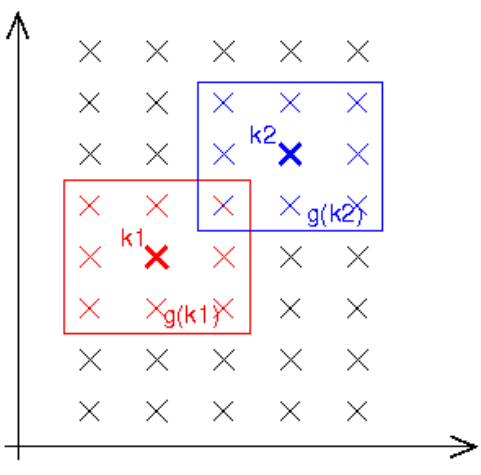
\includegraphics[width=3.5cm]{./grouplasso.png}
		\caption{Group-LASSO regression on two overlapping groups\footfullcite{sparsitykowalski2}}
		\vspace{-1em}
	\end{figure}
\end{frame}

\begin{frame}
	\frametitle{Tonal/transient separation with Group-LASSO}
	WMDCT\footfullcite{wmdct} + Group-LASSO -- ``audioshrink''\footnote{\url{https://homepage.univie.ac.at/monika.doerfler/StrucAudio.html}, \url{https://ltfat.github.io/doc/demos/demo_audioshrink.html}}
	\begin{figure}[ht]
		\vspace{-0.5em}
		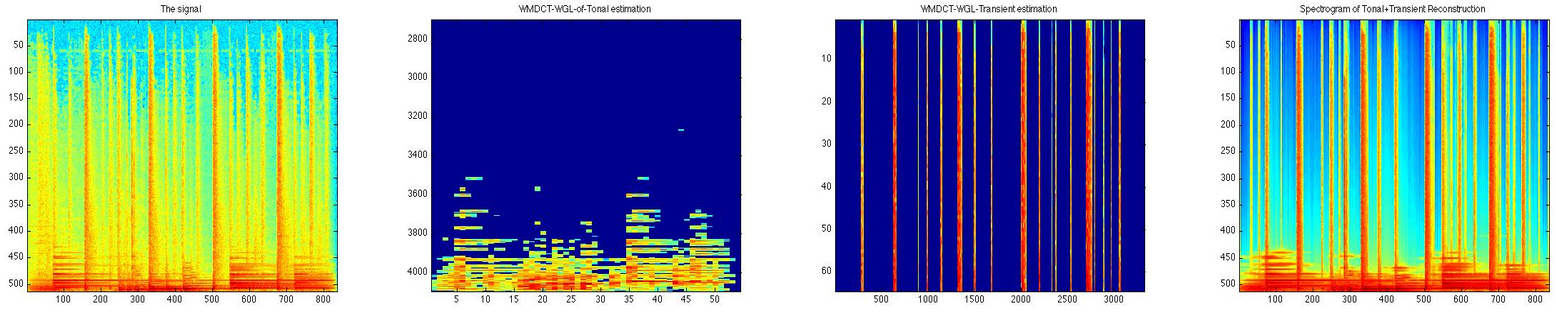
\includegraphics[width=11cm]{./wmdctjazz.png}
		\caption{Audioshrink for tonal/transient separation in jazz music}
		\vspace{-0.5em}
	\end{figure}
	Use 2 WMDCT transforms (wide + narrow window) + Group-LASSO to shrink input signal into significant coefficients in ``time'' and ``frequency'' groups. Example: \href{run:./mix.wav}{\faVolumeUp \ mix}, \href{run:./harm.wav}{\faVolumeUp \ tonal}, \href{run:./perc.wav}{\faVolumeUp \ transient}
\end{frame}

\begin{frame}[fragile]
	\frametitle{WMDCT tonal/transient dictionaries}
	\begin{figure}[ht]
		\vspace{-1em}
		\subfloat{\makebox[0.4\textwidth]{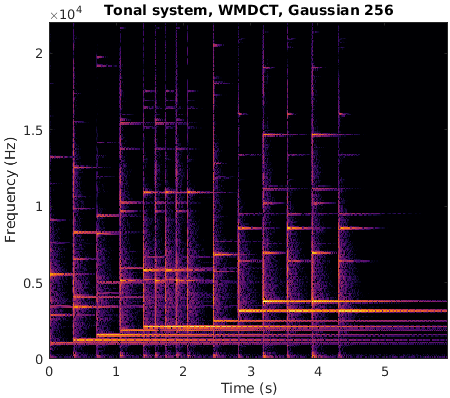
\includegraphics[height=3.5cm]{./glock_wmdct_tonal.png}}}
		\subfloat{\makebox[0.4\textwidth]{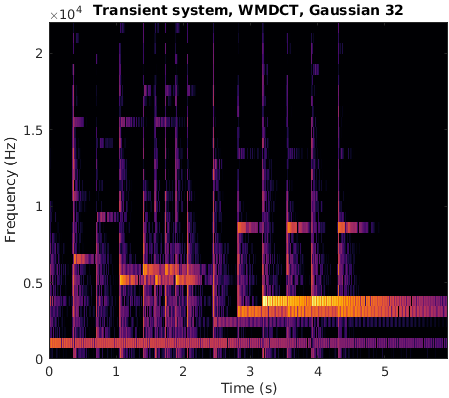
\includegraphics[height=3.5cm]{./glock_wmdct_transient.png}}}\\
		\caption{WMDCT + Group-LASSO shrink tonal/transient separation\footnote{\url{https://ltfat.github.io/doc/frames/franagrouplasso.html}, \url{https://ltfat.github.io/doc/demos/demo_audioshrink.html}}}
		\vspace{-1em}
	\end{figure}
	2 Gabor systems + \Verb#franagrouplasso#:
	\begin{quote}
		franagrouplasso(F,f,lambda) solves the group LASSO regression problem in the time-frequency domain: minimize a functional of the synthesis coefficients defined as the sum of half the $\mathit{l}_{2}$ norm of the approximation error and the mixed $\mathit{l}_{1}$/$\mathit{l}_{2}$ norm of the coefficient sequence, with a penalization coefficient lambda.
	\end{quote}
\end{frame}

\begin{frame}
	\frametitle{Lasso comparison for tonal/transient separation}
	Tonal layer is expected to be sparsely represented in the frequency domain, with emergent frequencies that may evolve slowly with time (i.e. almost horizontal lines of large MDCT coefficients). Lasso choices:
	\begin{itemize}
		\item
			E-LASSO (sparse within group) with the time label as group label
		\item
			G-LASSO (sparse across groups) with the frequency label as group label - \textcolor{red}{\textbf{bad choice}} because of the slow evolution in time of frequencies
	\end{itemize}
	Transient layer is expected to be sparse in time, but spread out in the frequency domain. Lasso choices:
	\begin{itemize}
		\item
			E-LASSO (sparse within group) with the frequency label as group label
		\item
			G-LASSO (sparse across groups) with the time label as group label -- \textcolor{ForestGreen}{\textbf{good choice}} because transients are sharply time-localized
	\end{itemize}
\end{frame}

\begin{frame}
	\frametitle{Transform to dictionary} 
	\begin{quote}
		Mallat and Zhang\footfullcite{dictionary1} proposed a novel sparse signal expansion scheme based on the selection of a small subset of functions from a general overcomplete dictionary of functions. Chen, Donoho and Saunders\footfullcite{dictionary2} published their influential paper on the Basis Pursuit, and the two works signalled the beginning of a fundamental move from transforms to dictionaries for sparse signal representation ... The terminological change enclosed the idea that a signal was allowed to have more than one description in the representation domain, and that selecting the best one depended on the task\footfullcite{dictionary}
	\end{quote}
\end{frame}

\begin{frame}
	\frametitle{Sparsity and entropy} 
	Sparsity and entropy are complementary concepts\\\ \\
	Given a signal $x$, its transform $w$, and probability mass function $p$:
	\begin{itemize}
		\item
			\textit{Sparsity, compressibility:} the property of concentrating most of the energy of $x$ in few coefficients of $w$
		\item
			\textit{Entropy, uncertainty:} the property of not concentrating most of the probability mass of $x$ in few atoms of $p$
	\end{itemize}
	For a given signal $x$, the uncertainty (randomness) of its elements defines the compressibility (compactness) of its coefficients $w$ in a given domain\footfullcite{pastor2015mathematics}\\

\end{frame}

\begin{frame}
	\frametitle{Time-Frequency Jigsaw Puzzle}
	\begin{enumerate}
		\item
			Create time-frequency ``super-tiles'' by superimposing a large window + small window Gabor analysis
		\item
			Use R{\'e}nyi entropy to set coefficients to zero where sound has more entropy than random white noise
	\end{enumerate}
	\begin{figure}[ht]
		\vspace{-0.75em}
		\subfloat[TF supertiles]{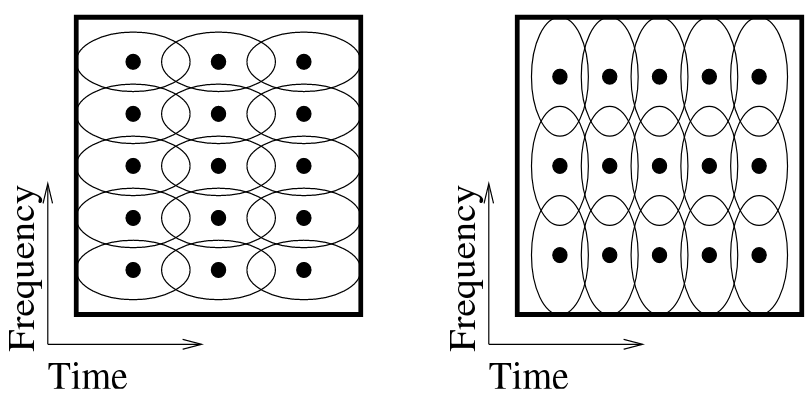
\includegraphics[width=5.25cm]{./tfjigsaw-supertiles.png}}
		\hspace{0.1em}
		\subfloat[Entropy criterion]{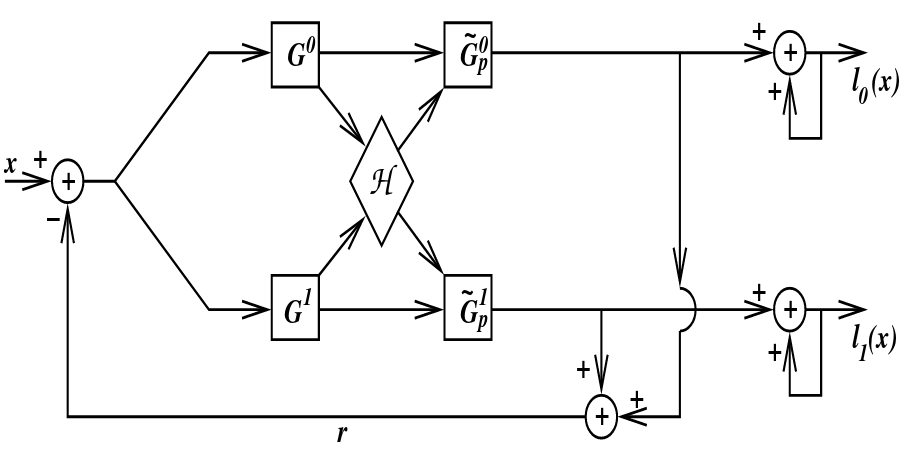
\includegraphics[width=5.25cm]{./tfjigsaw-entropycriterion.png}}
		\caption{TF Jigsaw Puzzle tonal/transient separation\footfullcite{tfjigsaw}}
	\end{figure}
\end{frame}

\note{
	\begin{itemize}
		\item
			i.e. good tonal/good transient
		\item
			high entropy = indicating sound is poorly represented
	\end{itemize}
}

\begin{frame}
	\frametitle{TFJigsaw}
	\begin{figure}[ht]
		\vspace{-1em}
		\subfloat{\makebox[0.4\textwidth]{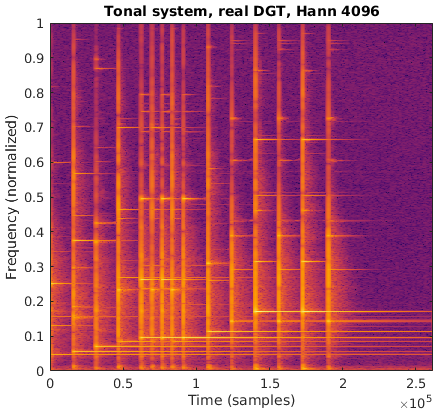
\includegraphics[height=3.5cm]{./glock_dgtreal_tonal.png}}}
		\subfloat{\makebox[0.4\textwidth]{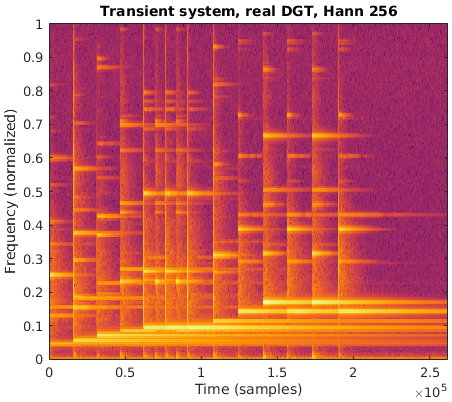
\includegraphics[height=3.5cm]{./glock_dgtreal_transient.png}}}\\
		\vspace{-1em}
		\subfloat{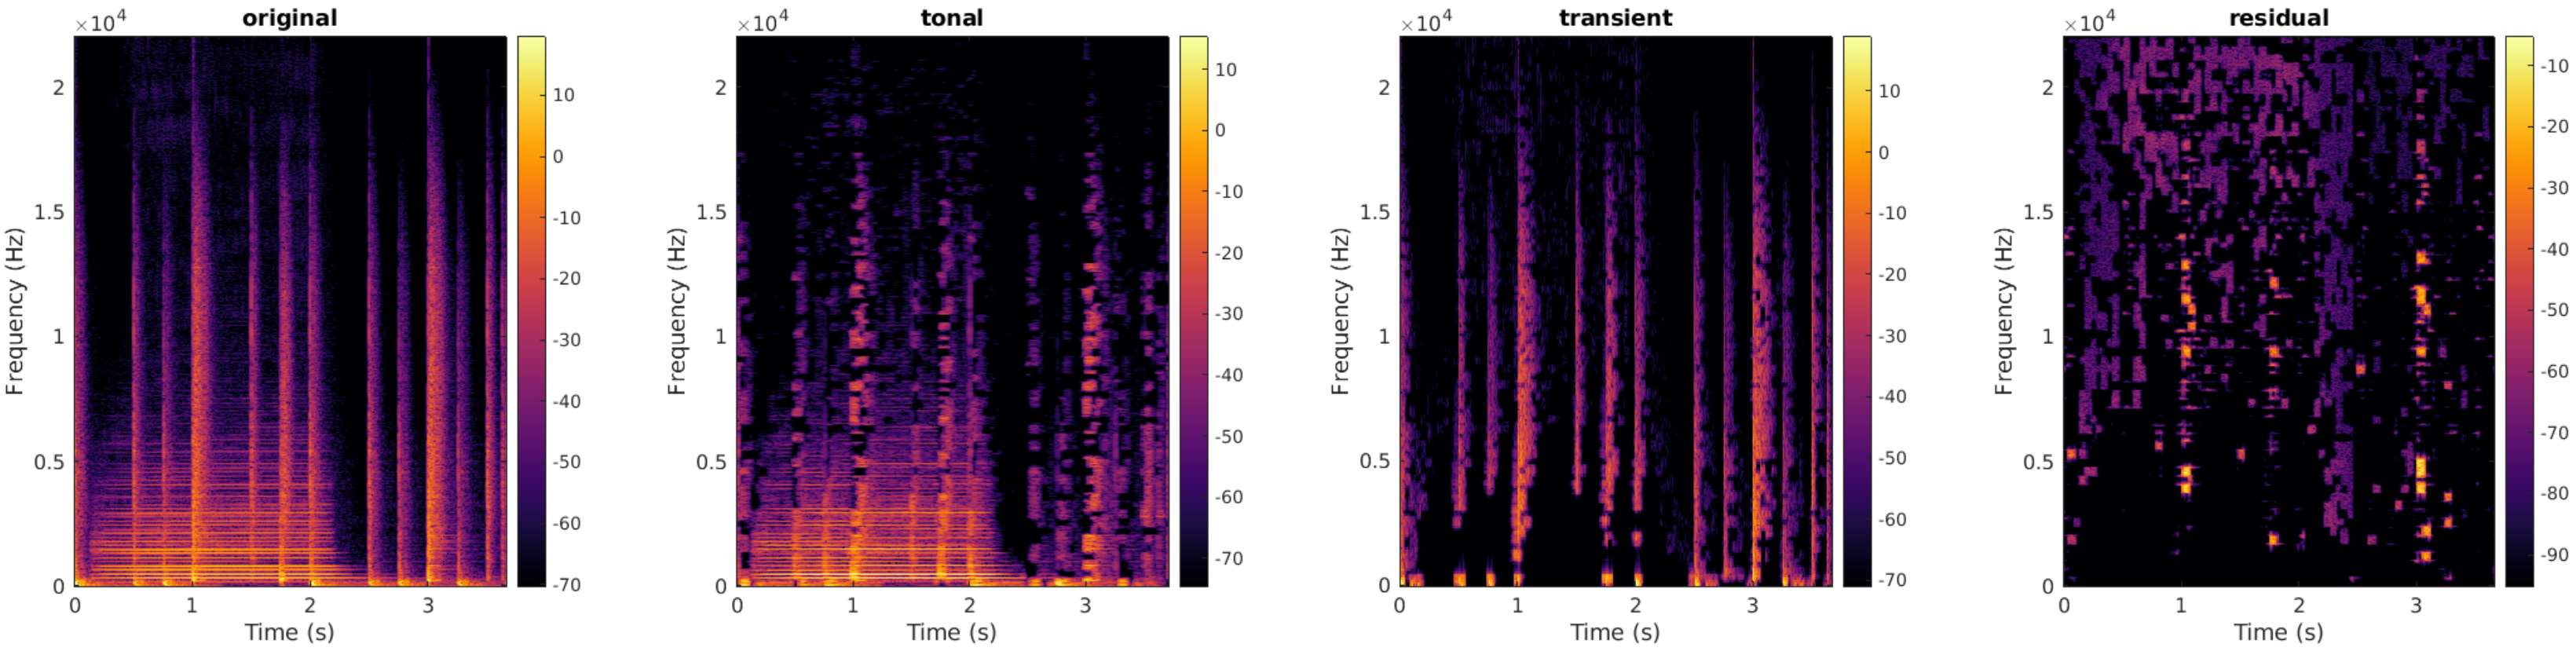
\includegraphics[width=11cm]{./tfjigsaw-sep-example.png}}
		\caption{TF Jigsaw Puzzle tonal/transient separation\footnote{\url{https://ltfat.github.io/doc/sigproc/tfjigsawsep.html}, \url{https://github.com/ltfat/ltfat/blob/master/demos/demo_tfjigsawsep.m}}}
	\end{figure}
\end{frame}

\end{document}
